\documentclass[11pt,a4paper]{article}
\usepackage[margin=2.3cm]{geometry}
\usepackage{graphicx}
\usepackage{booktabs}
\usepackage{tabularx}
\usepackage{array}
\usepackage{float}
\usepackage{xcolor}
\usepackage{fontspec}
\usepackage{ucharclasses}
\usepackage{hyperref}
\usepackage{bookmark}

\setmainfont[ItalicFont={Noto Sans CJK KR}]{Noto Sans CJK KR}
\newfontfamily\hangulfont[ItalicFont={Noto Sans CJK KR}]{Noto Sans CJK KR}
\setTransitionsForCJK{\hangulfont}{}{}

\tolerance=1000
\emergencystretch=3em
\hfuzz=2pt

\definecolor{titleblue}{HTML}{1F4E79}
\definecolor{softblue}{HTML}{F2F7FB}
\definecolor{softgray}{HTML}{F7F7F7}

\title{\textbf{Exp 4-2 업데이트 보고서}\\[0.4em]
\large Lie 군 관점에서 다시 정리한 회전 기반 KV-cache 양자화 결과}
\author{Boltzmann Attention / FOKVQ}
\date{2026년 4월 3일}

\begin{document}
\maketitle

\section{요약}

이번 업데이트의 핵심은 단순하다. 현재 결과는 ``FOKVQ가 baseline을 이긴다''는 논문보다, ``회전 기반 KV-cache 양자화를 어떤 수학적 문제로 봐야 하는가''를 정리하는 논문에 더 잘 맞는다.

확정적으로 말할 수 있는 것은 세 가지다. 첫째, K-space의 비등방성과 구조적 축 선택 효과는 실재한다. 둘째, GPT-2에서는 \texttt{PCA basis}가 \texttt{random}과 \texttt{identity}보다 확실히 낫다. 셋째, Qwen/GQA에서는 practical leader가 여전히 \texttt{kivi\_residual}이며, 단순 real rotation이나 초기 RoPE-aware 변형은 이를 넘지 못했다.

따라서 현재 결론은 다음과 같다. \textbf{Lie 군 기반 회전 선택 해석은 의미가 있지만, 그 해석이 자동으로 완성된 low-bit SOTA quantizer를 만들어 주지는 않는다.} 지금의 병목은 회전 존재 여부보다 어떤 generator가 살아남는가와 회전 후 quantizer가 충분히 강한가에 있다.

\section{Fact Base와 출처 정책}

이번 보고서는 아래 자료만 근거로 삼는다.

\begin{table}[H]
\centering
\caption{보고서의 근거 자료와 사용 정책}
\small
\begin{tabularx}{\textwidth}{@{}l l X@{}}
\toprule
\textbf{구분} & \textbf{현재 사용 여부} & \textbf{근거} \\
\midrule
\texttt{results/v3/gpt2-medium\_full\_quant\_ppl\_v3.json} & 사용 & 현재 레포에 남아 있는 GPT-2 v3 raw JSON \\
\texttt{reports/exp4\_2\_separate\_report\_ko.md} & 사용 & GPT-2 same-harness 표와 원격 raw artifact 경로를 함께 정리한 보고서 \\
\texttt{reports/exp4\_2\_autoresearch\_log.md} Iteration 24--29 & 사용 & 수정된 Qwen queue의 최종 수치와 해석이 남아 있는 작업 로그 \\
\texttt{results/v3/qwen2.5-7b\_full\_quant\_ppl\_v3.json} & 사용 안 함 & 과거 실패 런으로, hook/runtime error가 포함된 stale JSON \\
\texttt{/tmp/exp4\_2\_v3\_rotation\_smoke\_20260403/...json} & 제한적 사용 & 현재 harness wiring과 \texttt{benchmark\_meta} 기록 여부를 확인하는 smoke 전용 자료 \\
\bottomrule
\end{tabularx}
\end{table}

즉, 이 보고서에서 Qwen practical 표는 오래된 \texttt{results/v3/qwen2.5-7b\_full\_quant\_ppl\_v3.json}이 아니라, 수정 후 작업 로그와 별도 상태 보고서를 source of truth로 사용한다.

\section{질문별 요약}

\begin{table}[H]
\centering
\caption{질문, 의도, 결과, 현재 판단}
\small
\begin{tabularx}{\textwidth}{@{}l X X l@{}}
\toprule
\textbf{질문} & \textbf{의도} & \textbf{관찰 결과} & \textbf{현재 판단} \\
\midrule
\texttt{Q1. 회전 선택은 실제로 중요한가?} & basis effect 자체를 검증 & GPT-2 2-bit에서 \texttt{identity > random > PCA} 순서의 큰 차이 확인 & 지지됨 \\
\texttt{Q2. 현재 FOKVQ가 practical winner인가?} & low-bit main table에서 baseline 우위 확인 & GPT-2 2-bit, Qwen 3/4-bit 모두 strong control을 넘지 못함 & 지지되지 않음 \\
\texttt{Q3. GQA/RoPE에서 어떤 bias가 중요한가?} & 현대 모델에서 살아남는 구조 확인 & \texttt{kivi\_residual}과 \texttt{recent tail + structured prefix} 계열이 가장 안정적 & 부분 지지 \\
\texttt{Q4. 단순 RoPE-aware Lie 후보가 충분한가?} & 복소수/회전 해석의 직접 구현 검증 & \texttt{rope\_unitary}, \texttt{rope\_magphase}는 크게 실패 & 반증됨 \\
\texttt{Q5. 현재 harness는 새 가설을 시험할 준비가 되었는가?} & smoke-critic gate 확인 & self-test 통과, mechanistic smoke 통과, preset metadata 기록 확인 & 예 \\
\bottomrule
\end{tabularx}
\end{table}

\section{무엇이 바뀌었는가}

초기 문서군은 두 종류의 주장을 섞고 있었다. 하나는 ``PCA 기반 FOKVQ가 기존 방법보다 좋다''는 방법론 주장이고, 다른 하나는 ``회전 기반 양자화는 Lie 군 작용으로 볼 수 있고, 좋은 회전 선택이 핵심이다''는 해석 주장이다. 현재까지의 실험은 두 번째 주장을 더 강하게 지지한다. 그래서 이번 업데이트는 논문, 계획, 코드 모두를 그 방향으로 다시 정리한다.

\section{현재까지 검증된 사실}

\subsection{GPT-2에서의 basis-selection effect}

\begin{table}[H]
\centering
\caption{GPT-2 same-harness 2-bit 축 ablation (\texttt{topk=0.5})}
\small
\begin{tabular}{lr}
\toprule
\textbf{Basis} & \textbf{PPL} \\
\midrule
identity & 149.8334 \\
random & 52.9955 \\
FOKVQ(PCA) & 34.5466 \\
\bottomrule
\end{tabular}
\end{table}

이 표는 두 가지를 보여 준다. 첫째, \texttt{PCA basis}는 단순한 장식이 아니다. 둘째, 이 효과만으로 \texttt{KIVI-style} 또는 \texttt{turboquant-style}을 이기지는 못한다. 같은 main table에서 \texttt{FOKVQ}=34.5466, \texttt{KIVI-style}=27.7507, \texttt{turboquant-style}=27.7524였다.

\begin{figure}[H]
\centering
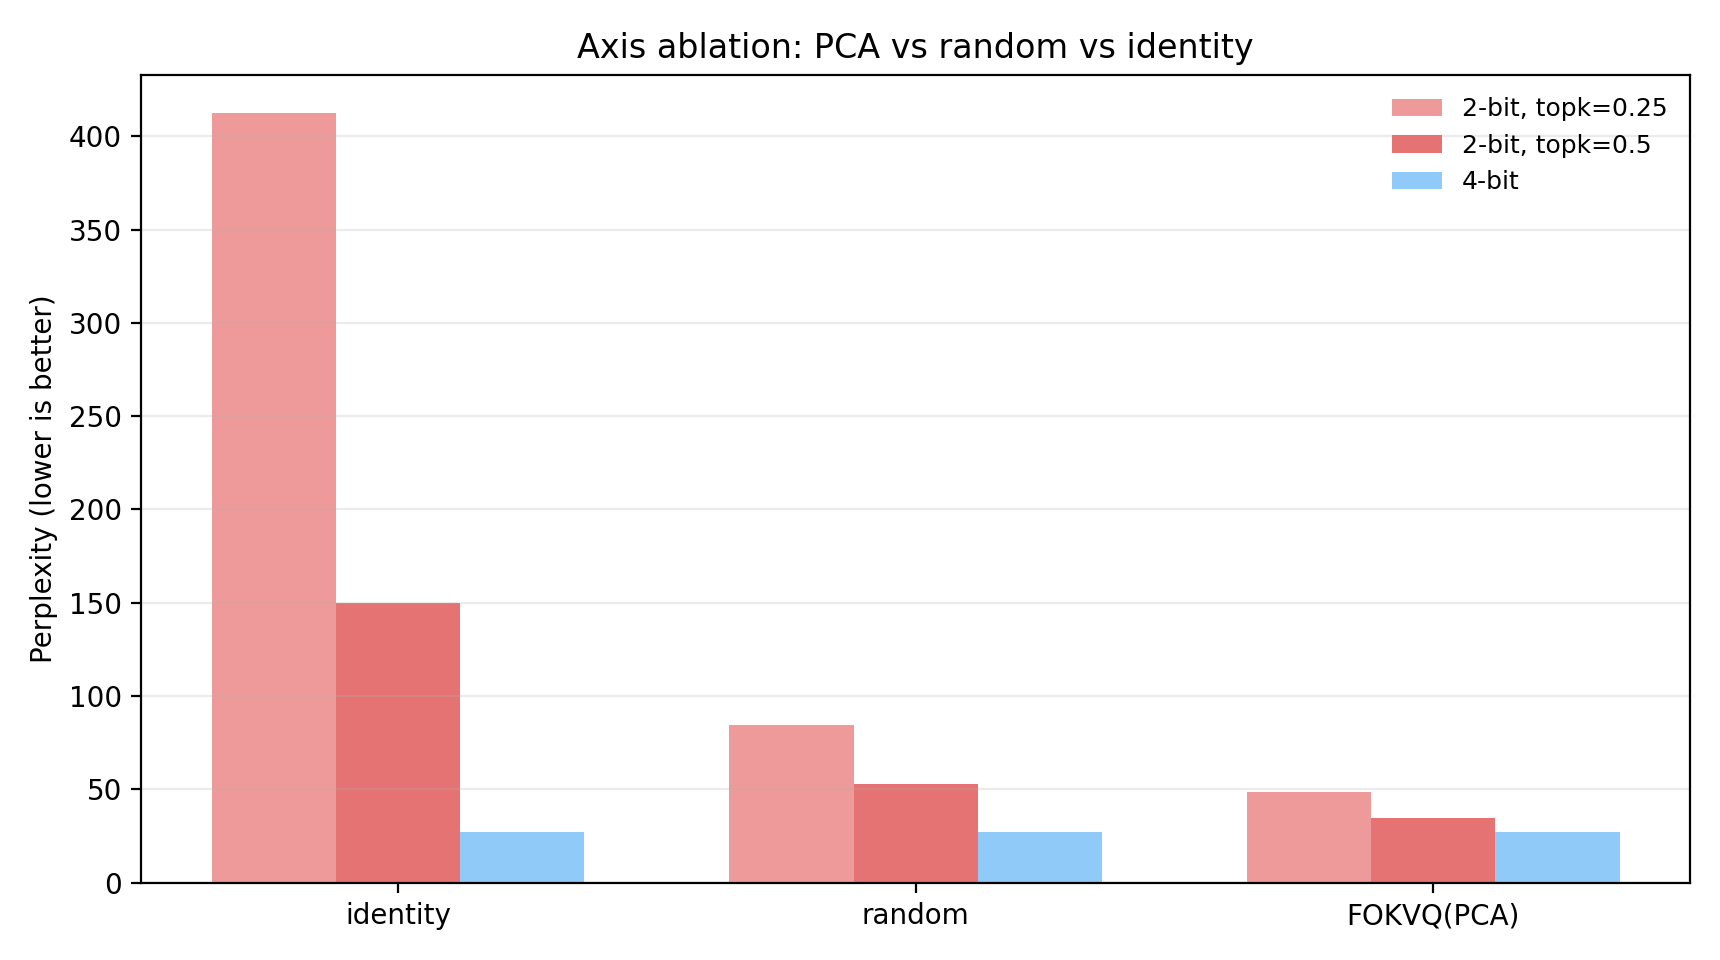
\includegraphics[width=0.88\textwidth]{figures/exp4_2_axis_ablation.png}
\caption{축 선택 ablation. 저비트에서는 \texttt{PCA basis}가 \texttt{random}과 \texttt{identity}보다 유리하지만, 그 효과만으로 strong baseline 우위를 만들지는 못한다.}
\end{figure}

\subsection{GPT-2에서의 4-bit 포화 구간}

\begin{table}[H]
\centering
\caption{GPT-2 same-harness 4-bit main comparison}
\small
\begin{tabular}{lr}
\toprule
\textbf{Method} & \textbf{PPL} \\
\midrule
FP16 & 26.8638 \\
KIVI-style & 26.8770 \\
uniform & 26.8983 \\
FOKVQ & 26.9954 \\
turboquant-style & 27.0020 \\
\bottomrule
\end{tabular}
\end{table}

\texttt{4-bit}에서는 거의 모든 방법이 붙어 있다. 같은 이유로 4-bit axis ablation에서도 \texttt{random}=26.9509, \texttt{FOKVQ(PCA)}=26.9954, \texttt{identity}=27.0862로 차이가 매우 작다. 따라서 현재 논문의 핵심 mechanistic evidence는 4-bit가 아니라 2-bit stress regime에 있다.

\subsection{Qwen에서의 practical ranking}

\begin{table}[H]
\centering
\caption{Qwen2.5-7B full-K quantization 16k run}
\small
\begin{tabular}{lrr}
\toprule
\textbf{Method} & \textbf{3-bit PPL} & \textbf{4-bit PPL} \\
\midrule
FP16 & 6.7544 & 6.7544 \\
kivi\_residual & 7.2060 & 6.7738 \\
turboquant\_rand & 7.5587 & 7.0212 \\
turboquant & 7.5671 & 7.0900 \\
quip & 9.1795 & 7.1394 \\
fokvq\_e2 & 8.7232 & 8.4917 \\
fokvq & 9.6555 & 7.4720 \\
\bottomrule
\end{tabular}
\end{table}

이 표가 말하는 것은 단순하다. Qwen/GQA/RoPE에서는 \texttt{recent residual tail}을 살리는 practical bias가 매우 강하다. 같은 이유로 \texttt{fokvq\_e2\_residual}은 plain \texttt{fokvq\_e2}보다 3-bit에서 좋아졌지만, 여전히 \texttt{kivi\_residual}과는 거리가 있다.

\subsection{초기 Lie 후보의 실패}

\begin{table}[H]
\centering
\caption{Qwen 2048 smoke: 초기 RoPE-aware 후보}
\small
\begin{tabular}{lrr}
\toprule
\textbf{Method} & \textbf{3-bit PPL} & \textbf{4-bit PPL} \\
\midrule
kivi\_residual & 6.5734 & 6.1431 \\
rope\_unitary & 14.3512 & 13.9959 \\
rope\_magphase & 750.0469 & 424.5279 \\
\bottomrule
\end{tabular}
\end{table}

이 결과는 ``RoPE-aware''라는 이름만으로는 충분하지 않다는 반증이다. pair-local 회전이나 단순 magnitude-phase 분해는 현재 구현에서 실제로 도움을 주지 못했다.

\section{지금까지의 해석}

이 결과들을 함께 읽으면 다음 구조가 보인다.

\subsection{이미 지지되는 해석}

\begin{itemize}
\item 회전 선택은 진짜 문제다.
\item 정적 basis choice는 quality에 영향을 준다.
\item PCA는 적어도 정적 회전의 강한 baseline이다.
\item GQA/RoPE에서는 recent tail + old prefix structured transform이 중요한 inductive bias다.
\end{itemize}

\subsection{아직 지지되지 않는 해석}

\begin{itemize}
\item 현재 FOKVQ가 완성된 practical winner다.
\item 임의의 Lie-inspired transform이 baseline보다 낫다.
\item reconstruction MSE를 줄이면 PPL도 자동으로 좋아진다.
\end{itemize}

특히 \texttt{fokvq\_lloyd}는 rotated-space reconstruction MSE는 줄였지만 PPL은 개선하지 못했다. 이 사실은 지금의 병목이 단순 scalar quantizer 교체가 아니라는 점을 보여 준다.

\section{벤치마크를 어떻게 다시 잡아야 하는가}

이 논문이 실제로 검증하고 싶은 것은 ``좋아 보이는 숫자''가 아니라 ``Lie 군 기반 회전 선택 가설''이다. 따라서 벤치마크를 네 층으로 나눠야 한다.

\begin{table}[H]
\centering
\caption{개정된 benchmark ladder}
\small
\begin{tabularx}{\textwidth}{@{}l l X@{}}
\toprule
\textbf{층위} & \textbf{현재 선택} & \textbf{역할} \\
\midrule
Quality & WikiText-2 full-K PPL & pure LM quality retention 측정 \\
Mechanism & axis ablation & \texttt{identity/random/PCA} 비교로 basis effect 측정 \\
Retrieval & NIAH depth sweep & position-sensitive cache geometry 유지 여부 측정 \\
External & optional long-context suite & B1--B3 안정화 이후의 일반화 \\
\bottomrule
\end{tabularx}
\end{table}

\section{코드와 프로토콜에서 바로 수정한 점}

이번 정리 과정에서 코드 정합성도 함께 점검했다.

\begin{enumerate}
\item \texttt{exp4\_2\_v3\_full\_quant\_ppl.py}에 \texttt{benchmark preset} 개념을 추가했다.
\item preset마다 \texttt{intent / hypothesis / verification focus}가 JSON에 남도록 수정했다.
\item \texttt{rotation\_mechanistic} preset에 필요한 \texttt{identity}, \texttt{random} basis가 v3 dispatch에 빠져 있던 버그를 수정했다.
\item local launcher가 기본 \texttt{python3}를 써서 \texttt{torch}가 없는 환경에서 실패하던 문제를 수정하고, 기본 interpreter를 명시적으로 고정했다.
\item launcher 출력 경로를 repo-level \texttt{results/}와 \texttt{reports/}로 정리해, 이후 보고서가 드리프트 경로를 참조하지 않게 했다.
\item 결과 JSON에 \texttt{generated\_at}, \texttt{hostname}, \texttt{cwd}, \texttt{git\_head}를 남기도록 수정해 provenance를 추적 가능하게 했다.
\end{enumerate}

수정 후 self-test는 통과했고, 작은 \texttt{rotation\_mechanistic} preset smoke도 정상 종료됐다. 단, 이 smoke는 wiring 검증일 뿐이며 scientific evidence로 해석하면 안 된다.

\section{다음 단계}

이제 autoresearch는 무작정 많은 표를 돌리는 방식이 아니라 아래 순서로 진행해야 한다.

\begin{enumerate}
\item \texttt{self-test} 통과
\item preset smoke 통과
\item \texttt{rotation\_mechanistic}에서 basis-level gain 확인
\item 그 다음에만 \texttt{ppl\_quality} 또는 \texttt{retrieval\_depth} full run
\end{enumerate}

현재 가장 타당한 active queue는 다음 세 가지다.

\begin{itemize}
\item \texttt{complex\_unitary\_residual}
\item \texttt{banded\_complex\_unitary\_residual}
\item \texttt{complex\_query\_metric\_residual}
\end{itemize}

이 셋 중 어느 것도 \texttt{random} 또는 plain \texttt{fokvq}를 넘지 못하면, 이번 논문에서 Lie 군 해석은 constructive method claim이 아니라 descriptive interpretation으로 남겨야 한다.

\section{결론}

현재까지의 결과는 부정적이지만 무의미하지는 않다. 지금 밝혀진 가장 중요한 사실은 어떤 회전이든 넣으면 좋아지는 것이 아니라, 회전 선택 문제와 quantizer 문제를 분리해서 봐야 한다는 점이다. GPT-2는 이 분리를 강하게 지지하고, Qwen은 practical winner가 어디에 있는지 냉정하게 보여 준다.

따라서 지금의 가장 좋은 논문 방향은 Lie 군 관점에서 회전 기반 KV-cache 양자화를 재해석하고, 그 해석이 어디까지 empirically 살아남는지를 정리하는 것이다. 그 위에서 추가 실험이 성공하면 method paper로 확장할 수 있고, 실패하더라도 분석 논문으로서의 가치는 유지된다.

\end{document}
